\documentclass[final]{cmpreport}

\usepackage{enumitem}
\usepackage{wasysym}
\usepackage{framed}
\usepackage{pgfgantt,rotating}
\usepackage{subfloat}
\usepackage{listings}
\usepackage{xcolor}
\usepackage{colortbl}
\usepackage{url}
\usepackage{hyperref}

\usepackage{color}
  \definecolor{lightgray}{rgb}{0.95, 0.95, 0.95}
  \definecolor{darkgray}{rgb}{0.4, 0.4, 0.4}
  \definecolor{purple}{rgb}{0.65, 0.12, 0.82}
  \definecolor{otherCode}{rgb}{1, 0.5, 0} % #FF7F00 -> rgb(239, 169, 0)
  \definecolor{blueCode}{rgb}{0, 0, 0.93} % #0000EE -> rgb(0, 0, 238)
  \definecolor{greenCode}{rgb}{0, 0.6, 0} % #009900 -> rgb(0, 153, 0) 
\usepackage{upquote}
\usepackage{listings}
\makeatletter
\lstdefinelanguage{HTML5}{
  sensitive=true,
  keywords={%
  % JavaScript
  typeof, new, true, false, catch, function, return, null, catch, switch, var, if, in, while, do, else, case, break,
  % HTML
  html, title, meta, style, head, body, script, canvas,
  % CSS
  border:, transform:, -moz-transform:, transition-duration:, transition-property:,
  transition-timing-function:
  },
  % http://texblog.org/tag/otherkeywords/
  otherkeywords={<, >, \/},   
  ndkeywords={class, export, boolean, throw, implements, import, this},   
  comment=[l]{//},
  % morecomment=[s][keywordstyle]{<}{>},  
  morecomment=[s]{/*}{*/},
  morecomment=[s]{<!}{>},
  morestring=[b]',
  morestring=[b]",    
  alsoletter={-},
  alsodigit={:}
}
\lstset{%
  % Basic design
  backgroundcolor=\color{lightgray},
  basicstyle={\tiny\ttfamily},   
  frame=l,
  % Line numbers
  xleftmargin={0.75cm},
  numbers=left,
  stepnumber=1,
  firstnumber=1,
  numberfirstline=true,
  % Code design
  identifierstyle=\color{black},
  keywordstyle=\color{blue}\bfseries,
  ndkeywordstyle=\color{greenCode}\bfseries,
  stringstyle=\color{otherCode}\ttfamily,
  commentstyle=\color{darkgray}\ttfamily,
  % Code
  language={HTML5},
  tabsize=2,
  showtabs=false,
  showspaces=false,
  showstringspaces=false,
  extendedchars=true,
  breaklines=true
}
\makeatother

\title{Building a Cross-Platform\\Mobile Game with HTML5}

\author{Joshua Barnett}

\registration{5939968}
\supervisor{Professor Andy Day}

\ccode{CMPC3P2Y}

\summary{
Creating cross-platform games is a necessity for aspiring developers. Indeed, the more platforms a game supports, the wider an audience the developer can reach, and therefore the bigger their potential for success. Nowhere is this more evident than in the mobile gaming market. However, the platform fragmentation associated with mobile devices impedes the development process, as tailoring an application to each different device is impractical, and, in most cases, extraneous. One attractive solution to this impediment is targeting the web platform that constitutes openness and inherent portability. This project aims to explore the web platform's pros and cons by researching the key technologies available for developers to  use. These technologies will then be assessed through the creation of a mobile game, and by rating the ease of creation and deployment when compared to conventional native development.

Full assessment of the field would require an analysis of both native and non-native development, but the scope of this project does not allow me to do both. Therefore, the focus of this project will be on HTML5 and the web platform. However, while HTML5 will indeed constitute the core of my analysis - this is what I have used to build my prototype mobile game - I will refer to native development from my personal observations and apparent evidences as a means to provide field for comparison and give depth to my examinations and conclusions. During the early years of my education, I taught myself how to draw and animate in Adobe Flash through watching online tutorials. I then learnt ActionScript and used this new skill to make games that were sold for sponsorship on various Flash gaming portals. Nevertheless, since that time, the industry has been shifting away from using third-party proprietary plugins in favour of open technologies such as HTML5. I feel this project will encourage me to research and learn these emerging technologies, and the knowledge gained will provide me with a strong footing for my desired career in industry.
}
\acknowledgements{
I would like to thank Professor Andy Day for supporting this project and its fluctuating nature. Thank you, also, to my parents Jane and Paul for cultivating my creative characteristics while enabling my technical skills, as well as to Elise Lanteri for her superior grasp of English grammar and the written word.
}

\begin{document}

\section{Introduction}
\label{sec:intro}

During the past five years, the popularity of mobile devices has been increasing. These devices have become one of the foremost ways in which the modern world consumes media and entertainment. Original equipment manufacturers (OEMs) such as Apple, LG, Nokia, and Samsung, have become progressively competitive in producing better mobile devices for the global market, generating a variety of them in the process. This growing market constitutes a large audience for mobile applications, which conscientious developers aspire to target. However, in order for a mobile application to succeed in such a competitive and saturated market, it is a necessity that they support as many devices as possible; the more devices an application supports, the wider an audience it can reach. Now, currently, this is an arduous process, as each mobile device falls into a subset of operating systems and hardware specifications. Each operating system has a different application programming interface (API), which is made accessible through its corresponding software development kit (SDK). Hence, for a developer to target each operating system `natively', the development of the application must vary and be adapted. This native adaptation process is an inefficient approach to cross-compatible mobile game development. It requires more time, more people, and, consequently, more money. At the core of this project's research is the exploration of a solution to this deterrent that developers have to face.

The Open Web Platform (OWP), in essence, is a collection of open (royalty-free) technologies that can be used for application development. The standards for these technologies are defined by the World Wide Web Consortium (W3C), in order to standardise and maximize a consensus amongst its members. Web applications built with these technologies benefit from the inherent portability of the Web, which means that they can be universally executed and distributed amongst a wide range of devices. Modern mobile devices fall into a subset of this range, as they contain essential software, such as web browsers, that can render and run web pages used to deliver the OWP. This makes the OWP an appealing free alternative to that of developing natively for each mobile operating systems, as the requirements for cross-compatibility are minimized.

HyperText Markup Language (HTML) is the corner stone technology of the OWP. Its purpose is to specify the content of a web page. The fifth iteration of HTML (HTML5) has further broadened the types of content that it can deliver, now allowing for the definition of rich interactive content such as audio, video, and a graphics within the page. HTML5 and its associated technologies can be leveraged by developers to create mobile games that support the variety of mobile devices. This project will focus on the usage of HTML5 and its companion technologies in mobile game development. In order to carry out my analysis, I have decided to build a game using HTML5, so that I could, along the way, assess the ease of development and deployment, as well as the difficulties arising from it.

\section{Background}

\subsection{Primer}

HTML5, as defined by the World Wide Web Consoritum \citep{W3C2}, is ` ... the 5th major revision of the core language of the World Wide Web'. However, the Web Hypertext Application Technology Working Group \citep{WHATWG} have recognised that `the term ``HTML5'' is widely used as a buzzword to refer to modern Web technologies'. This usage of ``HTML5'' as an umbrella term has been influenced by adoption and integration of existing widespread technologies into the W3C specification, encouraged by the design principles that underlie its development \citep{Keith}. In practical terms, this means that when an emerging technology becomes widely supported by the web development community and the web browser vendors (such as Google (Chrome), Apple (Safari), and Mozilla (Firefox)), it becomes a candidate for adoption into the specification. Notable examples of this happening early in HTML's development are the inclusion of \texttt{<style>} and \texttt{<script>} tags, which are commonly used to reference or embed Cascading Style Sheets (CSS) and ECMAScript (commonly known as JavaScript (JS)). These technologies are now key components of modern web applications.\footnotemark[1]

\footnotetext[1]{``Linux'' has similarly been distorted as an umbrella term when referring to Linux based operating systems such as Debian, Fedora, and Ubuntu. The literal use of ``Linux'' refers to the open-source kernel which lies at the heart of these distributions, but it alone does not represent a full operating system.}

Web browsers are client-side applications which let users view and navigate web content. This content is typically hosted on web servers that communicate with the web browser through the Hypertext Transfer Protocol (HTTP). Once the browser has received an initial HTML web page, it begins the process of parsing and rendering it. The parsing process also includes locating and requesting any additional resources that pertain to the web page, such as multimedia content, styles, and scripts. Once all of the relevant resources have loaded and are present client-side, the browser can begin fully rendering the page and the defined contents. This basic routine of web page acquisition also applies to HTML5 applications, as they often revolve around a root web page that acts as an entry point similar to that of \texttt{Main}, in languages such as Java and C++. Unfortunately, this delivery method has a few drawbacks when compared to that of native mobile applications: first, the user must have Internet connectivity to access the application, and they then have to launch a browser and navigate to the web address where the application is located. These shortcomings are arduous tasks for the average mobile consumer, as they are accustomed to acquiring applications through a centralised store, where applications are nicely categorized and presented, making comparison and browsing easy for the user. Once they have selected and installed an application, it can be launched through an icon created on the operating system's GUI (Graphical User Interface). `Offline \& Storage' technologies introduced as part of HTML5 are now assisting developers in circumventing the foremost of these issues, by letting them cache their application's files through the HTML5 Application Cache, as well as storing persistent data through HTML5 Local Storage. Mobile OSs such as Android and iOS are also rolling out support for the creation of web shortcuts on the native GUI, allowing them to sit alongside native applications. These strives are rapidly putting HTML5 applications on equal footing with native application presentation. Nevertheless, the barrier for entry is still too high for a casual user who is oblivious to applications outside that of the conventional centralised application stores. Until there is more support for HTML5 applications in the main application stores, another common workaround for developers is to package the HTML5 application within a native application, as this can create a native web view through the operating system's API, which in turn can be used to render the embedded HTML5 application. This helps blur the line between HTML5 and native mobile applications, and delivers the same installation and launch experience that users are acquainted with. These kinds of applications are referred to as `Hybrid' mobile applications, as they encompass advantages of both HTML5 and native applications' features. `Hybrid' development also helps safe guard web developers from some of the cross compatibility issues that come from supporting multiple browsers, by bundling a selected web view or browser on which their HTML5 application is executed.

Getting a HTML application to render and function consistently across a range of different web browsers can be a huge undertaking. As noted in section~\ref{sec:intro}, this task has grown exponentially with the introduction of mobile devices and their combinations of OS and web browsers. Each unique variation has the potential to produce bugs and quirks. While the HTML5 specification was being developed, much of the newly introduced features were implemented and experimented with at the discretion of the browser vendor. This has led to inconsistent support for these features across web browsers, as each vendor interprets the specifications differently while implementing them at varying rates. Developers must be aware of the idiosyncrasies between web browsers to ensure compatibility. Often, a developer will either limit their browser support scope and take full advantages of new features, or compromise and use polyfills, also known as a shims, to provide legacy support. A polyfill is often referred to as a code snippet that substitutes the lack of a future API by utilising existing features to mimic that of their final implementations \cite{Lawson}. Nevertheless, even after polyfilling feature gaps, there will still likely be unforeseen bugs that will prompt further testing and debugging. As I allude to in my introduction, the most reliable way to ensure compatibility is to physically test all browsers and mobile devices which the developer intends to support, but this solution is often impractical, especially with time, funds, and workforce limitations. The next best alternative is device emulation or investing in established cloud services that specialise in this method of testing.

\subsection{Theory}
When designing any game, a developer must constantly have the player in mind, as it is paramount that the player enjoys their participation in the game experience. Enjoyment can take many forms, but in the majority of the cases, it will ultimately boil down to the player obtaining satisfaction from playing and learning. Typically, this is achieved when successfully emulating a mental model akin to that of the game's underlying flow and structure. This allows for the player's prediction of causes and effects that take place within the game's system \citep{Cook}. Mobile gaming is a new platform which brings with it a new set of challenges for developers. One of these is delivering sufficient feedback to the player, whether it is visual or audible. The device is restricted by its hardware (compact screens, small speakers), and this can make the process of delivering feedback difficult, as, often, feedback is given to the player through these visual and audible means. Moreover, often, a player's attention is dedicated to another task (watching TV, travelling, etc), while they are playing, because they are multitasking. This requires that visual information be  extremely clear and easily understandable.

\subsubsection{Interface}
The choice of interface should be highly weighted relative to the context of the game system. For instance, a real-time game system would not be suited to that of a touch interface that simulates a conventional input system such as buttons (unless highly simplified). This is because it lacks tactile feedback and indirectly effects gameplay, creating a sense of incoherence in the user's experience. This method, however, could be applicable in the context of non-gameplay sections like menu navigation and non real-time game systems, such as turn-based game genres \citep{XuBradburn}. These systems, since they  involve no emphasis on player reaction time, lend themselves to such interface methods. One advantage to this approach is the omission of a tutorial, as most players are accustomed to such conventions.

A better route still is to provide an intuitive means of interface with the game system, that could enhance the game experience. Good examples of touch interfaces often take a minimal approach, consisting of few touch gestures. This has substantial benefits over that of the simulated. Angry Birds\footnotemark[2] is a classic example of an intuitive touch interface, as the gestures made by the player have direct correlation to visual feedback on the screen. Once the gesture is made, the game system simply uses your interaction as the seed of entropy that is then played out (using a physics engine), all the while allowing the user to clearly observe the causes and effects in the game system. Their interaction only formed the initial section of the game loop, and for the rest of time was not obscuring the visual feedback.

\footnotetext[2]{\url{http://www.angrybirds.com/} - Accessed October 2013}

\subsubsection{Methodology}
User-centred design (UCD) is an interesting approach to mobile game design. Instead of relying solely upon the experience and vision of designers, it considers the potential future players of the game to be the core design informant. At the core of any game design process is the objective to create a meaningful game experience for the player. Two key factors in achieving this are discernibility - providing the player feedback on their actions - and integration - showing the player their actions and their outcome in the larger context of the game system.

One positive effect of this perspective on game design is the fact that it avoids the potential pitfalls that stem from the designers themselves and their commitment to their game. Designers can have a tendency to ``fall in love'' with their own game ideas, as the game often originates from their own desires, namely, from what they personally look for in a game experience. Such approaches may misrepresent what the user base wants from their game experience, since it suffers from a lack of wide initial feedback and criticism. In other words, the design process should be a means to combine logic and information, in order to form satisfactory choices on which to base a game's blueprint. The information on which the game's logic is built can be yielded from a variety of sources: research literature, statistical data, player feedback and the designer's own input \citep{ErmiMayra}.

\subsubsection{Mechanics}
`Game mechanics are rule based systems or simulations that facilitate and encourage a user to explore and learn the properties of their possibility space through the use of feedback mechanisms.' \citep{Koster}. Games are engineered to provide enjoyment and a sense of satisfaction for the user. The games check this through recording a player's performed action, which in turn causes an effect in the game space. The player then receives feedback, often in the form of rewards or new tools which can then be used in the same or newly introduced game mechanics. Human behaviour has made this a good model because we have evolved through our increasing learning capabilities. The brain's reward centre will release chemicals (dopamine) that encourage such actions during the learning process.

\citet{Skinner} proved with his operant conditioning chamber that not only is it possible to condition human reactions, but it is also possible to condition human volition and change the way users make choices. Many successful games that exist in today's market are built on this principle and can sometime exploit its power over their audience. Operant conditioning experiments have shown that to get a player to engage in an activity, there must be some sort of feedback that the player takes pleasure in such as a reward. Nonetheless, it has also shown that the best way to get the player to repeat the activity is not to provide feedback too consistently. Instead, having the feedback delivered at random intervals or at set time periods has shown to be far more effective.

Games such as World of Warcraft\footnotemark[3] (WoW) and various social games have manipulated this human characteristic beyond their initial novelty. An example of that would be when a player has reached the ``end-game'' (reaching the maximum character level) in WoW; the key activities that are left to engage in are ``raids''. These are large-scale game scenarios that require several participants to progress through various virtual dungeons. Most of these dungeons have character class specific rewards that are delivered upon the defeat of a boss. These rewards, however, have a randomised probability of occurring, which bares significant similarities with that of the operant conditioning experiments. This game design methodology is not exclusive to that of large scale experiences. It can also be applied in a very simplistic context. Examples like Solitaire\footnotemark[4] and Candy Crush Saga\footnotemark[5] have infrequent reward systems for the player, which conditions them in a similar way. Nevertheless, though such experiences may be engaging for the player, this does not make them compelling forms of play \citep{ExtraCredits}.

\footnotetext[3]{\url{http://eu.battle.net/wow/en/} - Accessed October 2013}
\footnotetext[4]{\url{http://en.wikipedia.org/wiki/Solitaire} - Accessed October 2013}
\footnotetext[5]{\url{http://about.king.com/games/candy-crush-saga} - Accessed October 2013}

\section{Technologies}
The technologies used during the development of the HTML5 mobile game were researched and discovered as they were required. Instead of recounting them during section~\ref{sec:dev}, this section will be dedicated to explaining them independently, first to keep the report organised, and second, so they can be referred to when necessary, without extended explanation.

\subsection{Languages}

\subsubsection{Cascading Style Sheets (CSS)}
`CSS is a stylesheet language used to describe the presentational semantics of a document written in a markup language like HTML' \citep{Neilson}. Web browsers interpret this style markup when they encounter it in the form of \texttt{<style>} tags present in the web page, that may enclose or reference files containing CSS. The markup CSS uses involves using selectors and rules, to define how and where the browser should render an element. There are several basic principles that CSS uses; for instance, concepts such as document flow and the box model to structure a web page. Document flow is, essentially, the order and position in which the elements should appear on the web page, as defined by style attributes such as \texttt{display} and \texttt{position}. The box model is what wraps the content contained in an element, which can be manipulated through style attributes such as \texttt{width}, \texttt{height}, \texttt{padding}, \texttt{border}, and \texttt{margin}. CSS can also define the aesthetics of an element using color, gradients, borders, and filters, as well as the font properties that text within an element should obey.

The latest iteration of CSS specification (CSS3), which came about as part of the HTML5 platform, introduced some useful features that assist in cross-platform development like \textit{Media Queries}, which allow for conditional styles relative to screen resolution and density. These are  frequently used in web development to create responsive website designs that will adapt and scale to any form factor. Another useful additional feature was that of 3D transforms,  which enables document elements to be positioned, rotated, and scaled in three-dimensional space. This feature has been in development for awhile, and, as a result, it has been implemented in most mobile browsers under vendor prefixes, because it was considered `experimental' for a long time. Many mobile browsers also support GPU (Graphics Processing Unit) acceleration, for elements that have 3D transformations applied to them.

\subsubsection{JavaScript}
JavaScript is the most popular programming language to date (see figure \ref{ranking}). Every web browser today ships with a JavaScript interpreter, making it extremely portable and widely executable. JavaScript has been standardised under the alias ECMAScript (ECMA-262), the current version of which is 5.1\footnotemark[6]. However, the JavaScript pseudonym (a hangover from its forerunner) has become the preferred way to reference the language. JavaScript was originally created by Brendan Eich at Netscape as a way of making the newly added Java support in Netscape Navigator more accessible to non-Java programmers \citep{Champeon}. Since then, it has grown to be the most widely supported  language on the Web and is a core building block of modern web development.

\footnotetext[6]{\url{http://www.ecma-international.org/publications/standards/Ecma-262.htm} - Accessed February 2014}

\begin{figure}[h!]{The RedMonk Programming Language Rankings: January 2014 \label{ranking}}
  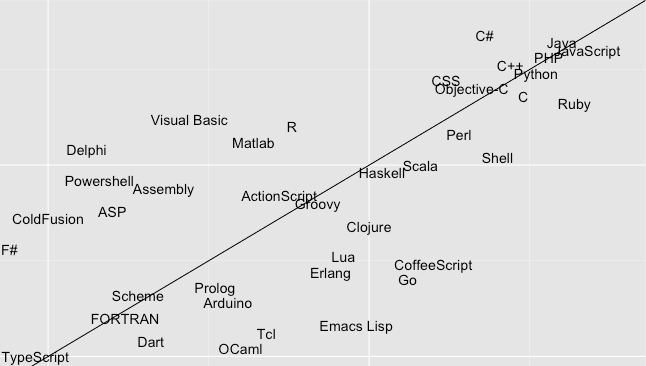
\includegraphics[width=1.0\textwidth]{lang-rank-114-wm.png}
  \begin{tablenotes}
    \item x-axis: Popularity Rank on GitHub (by \# of Projects)
    \item y-axis: Popularity Rank on Stack Overflow (by \# of Tags)
    \item Source: \url{http://redmonk.com/sogrady/2014/01/22/language-rankings-1-14/}\\Accessed February 2014
  \end{tablenotes}
\end{figure}

 In its current state - ECMAScript 5.1 - JavaScript is an underwhelming language, especially when compared to more mature languages like C++ or Java. Indeed, it lacks native support for object-orientated features such as inheritance, generics, and abstraction. As afore mentioned, JavaScript was never intended for use in large-scale development projects, but due to its inherent portability, it has become widespread and has had to bolt on improvements to keep up with trends. Until its apparent deficiencies are rectified and standardised in its forthcoming iterations (ECMAScript 6/7), developers have to overutilise its strengths, such as being loosely typed, functions as objects, dynamic objects, and literals \citep{Julian}. There are many development tools, such as transpilers, designed to alleviate some of these gaps in feature support, as well as full blown alternatives such as Google's Dart. These technologies can iterate faster than that of heavily standardised languages like JavaScript. The lengthy process of web language standardisation is a side effect of being open and having many parties contribute to the design and development of the language specification, but this long cycle does help ensure a consensus and long term stability.

One big hindrance of utilising JavaScript in large scale development is the lack of a modular design pattern. Typically, JavaScript is created as separate \texttt{.js} text files that are then referenced in a \texttt{.html} document by \texttt{<script>} tags. When the web browser finds scripts linked by these tags, it will request them from the web server and inject them into the document once loaded. This presents a few problems for large and complex web applications that often require many scripts, each having to be requested and loaded synchronously. Every one of these request has an overhead, which is compounded when a vast quantity are being made. This can lead to suboptimal load times.

To combat this problem a developer could attempt to write all their code in one \texttt{.js} file. This file can quickly become colossal, making it difficult to manage and refactor, especially on large scale projects. Alternatively, the developer can split their code into several \texttt{.js} files that will all have to be referenced by a corresponding \texttt{<script>} tag. Therefore, the more organised the codebase becomes, the more requests the browser has to make. The developer also has to micromanage these \texttt{<script>} tags to ensure their ordering is correct. The ordering is important because one script could be referencing another that has not yet been loaded, thus causing runtime errors. This approach also presents issues when attempting to introduce software engineering best practices such as unit testing, as the interdependencies between these scripts are not clearly defined.

There are a variety of libraries that offer solutions such as RequireJS\footnotemark[7], HeadJS\footnotemark[8] and yepnope.js\footnotemark[9]. After testing and evaluating some of these libraries, Browserify\footnotemark[10] presented itself as the simplest and the most supported amongst the Node.js community. Browserify enables developers to write their JavaScript code in numerous files, and when one file requires another it can be injected via the \texttt{require(`example');} function. Once a developer has written all their code, they can recursively bundle all their modules starting with a root module similar to that of a main class in conventional programming languages. This provides the developer with a good compromise, as all their code will be built into a single \texttt{.js} file (including their external libraries), while allowing for easy management and refactoring of their core codebase through individual source files.

\footnotetext[7]{\url{http://requirejs.org/} - Accessed January 2014}
\footnotetext[8]{\url{http://headjs.com/} - Accessed January 2014}
\footnotetext[9]{\url{http://yepnopejs.com/} - Accessed January 2014}
\footnotetext[10]{\url{http://browserify.org/} - Accessed February 2014}

Most might think that this will in turn cause complications when debugging, as when the code breaks, it will do so in the colossal \texttt{.js} file that the browser is running. This is where source maps come in. Source maps provide linkage between the original \texttt{.js} source files and their bundled counterparts making breakpoints and stepping through code painless \citep{Seddon}. This process can also be made seamless by Watchify, which automatically recompiles the Browserify bundle whenever a module file has been updated. This allows for the developer to work on their original source files, and, as soon as the file has been saved it has rebuilt the bundle ready to be reloaded in the browser for testing. After the modules have been bundled, a further step, called `minification', involves taking legible JavaScript and compressing it down into its most minimal form by removing unnecessary characters such as a whitespace and shrinking instance names. This process can further decrease the \texttt{.js} file size, making load times marginally faster while also partially obfuscating the original code from prying eyes.

\cite{Hanselman} stated an intriguing opinion that JavaScript had become akin to an assembly language for the web, which is the impression a lot of people get when taking a peek at the source of popular website such as Google or Facebook. This is somewhat understandable, given the that JavaScript is as `low-level' as developers can get when programming for the web. However, a fortunate side effect of being closely tide with the web is that it has now become one of the most portable languages to date, because every web enabled device has a browser, and every browser has a JavaScript virtual machine. This makes JavaScript a very cross-platform language to develop games with, which, since I have explained that reaching a wide audience is key when attempting to maximise chances for success, is a strong advantage.

\subsubsection{Google Dart}
Google's Dart ``is a new platform for scalable web app engineering'' which comes in the form of several tools. First, there is Dart the language, which is an alternative to writing plain JavaScript with a host of additional built-in and libraries language features akin to Java \citep{Fortuna}. Second, there is DartVM, a virtual machine that comes as a standalone program and also happens to be embedded in the Google Chrome browser. The DartVM works similarly to a typical JavaScript virtual machine with the difference being it interprets \texttt{.dart} code instead of \texttt{.js}, and with significant performance advantages \citep{Schneider}. Lastly, the dart2js compiler appeared, which is effectively a backwards compatibility tool to ensure that any application created on the Dart platform will still work through conventional means.

\subsubsection{Microsoft TypeScript}
Microsoft's TypeScript is, by its creators' admission `a typed superset of JavaScript that compiles to plain JavaScript', which makes it very flexible alternative. This effectively means that one can continue to write plain JavaScript, and no restrictions will be imposed by the TypeScript transpiler. This helps greatly if a developer already has a large JavaScript codebase that they wants to utilise during the development of a large scale application. TypeScript offers some of the inherently missing language features of JavaScript such as type annotations, classes, interfaces and modules\. There are also plans to support ECMAScript 6 features once it becomes the standard. Another positive remark about the output produced by the TypeScript transpiler is that it produces rather legible JavaScript, making it easy to see the relationships between the source and target languages.

Because the compile target of these transpilers is JavaScript, it is possible to take advantage of them when developing mobile web applications such as video games. When I first started developing my project, TypeScript was the target language because it was syntaxitcally similar to that of ActionScript 3, which is where my background lies. However, due to the immaturity of the project at the time and a lack of core JavaScript knowledge on my part, it was later ditched, as time constraints prevented the investment of fully learning its quirks. Also, it felt that working at this level of abstraction could potentially lead to delays when debugging later in development. Nonetheless, as of \textit{April 2014} close to the time of writing, the specification for TypeScript 1.0\footnotemark[11] has been finalised and its current status is \textit{stable}. Going forward after this project I am eager to re-evaluate it, since it now has had time to mature.

\footnotetext[11]{\url{http://www.typescriptlang.org/Content/TypeScript\%20Language\%20Specification.pdf} - Accessed May 2014}

\subsection{Visuals}

\subsubsection{The Document Object Model (DOM)}
`The Document Object Model is a platform- and language-neutral interface that will allow programs and scripts to dynamically access and update the content, structure, and style of documents. The document can be further processed and the results of that processing can be incorporated back into the presented page.' \citep{W3C3}. A web browser will create a DOM when parsing the elements and tags found in static HTML documents. This allows the browser to easily interpret relations between the content in the web page and use this information to render it appropriately. While in memory, these page elements, now represented as objects, are no longer static, which allows technologies such as JavaScript to manipulate and interact with them. Many web applications rely on the DOM's JavaScript API in order to deliver rich interactive user experiences. For instance, Gmail, is a SPA (single-page application) that makes heavy use of this API. SPAs have significant advantages over that of traditional web pages as they can provide seamless user experiences, similar to that of desktop applications. Instead of navigating between web pages through links that each request separate web pages, they manipulate the initial web page and load its required content and data in the background, displaying it when ready by weaving it into the current page context. This technique can help shrink load times by only requesting necessary data and reusing existing visual elements \citep{Takada}.

\subsubsection{HTML5 Canvas}
Canvas element is probably the most significant feature that was introduced in HTML5, especially for game developers. It finally enables developers to do interactive and dynamic graphics natively in the browser, without third-party plugins.

The new \texttt{<canvas>} element defines a graphics layer in a HTML document that can be manipulated and drawn to through a JavaScript API. Although this has been used in the context of desktop web applications to great effect, it has suffered from performance issues on mobile browsers. This is often due to being limited to software rendering that only makes use of the device's CPU. Nevertheless, the performance of mobile devices has been increasing in recent years, with an emphasis on GPU development \citep{Lin}. This has led to browser vendors adding support for GPU accelerated rendering on mobile devices in places that use complex effects such as CSS3.

Utilisation of these faster processors with the canvas element has only just started to become common place. There are many ongoing software projects with a focus on accelerating the HTML5 canvas using the mobile device's GPU. Unfortunately, there is a lack of cross platform open-source projects that tackle this issue. Ejecta is one of such projects, but it currently only supports iOS. Finally, the hybrid mobile application framework Apache Cordova\footnotemark[12] also provides an accelerated canvas through a plugin called FastCanvas\footnotemark[13].

\footnotetext[12]{\url{https://cordova.apache.org/} - Accessed October 2013}
\footnotetext[13]{\url{http://plugreg.com/plugin/phonegap/phonegap-plugin-fast-canvas} - Accessed November 2013}

\subsubsection{WebGL (Web Graphics Library)}
WebGL is a distillation of the popular OpenGL, which makes GPU accelerated rendering in the browser a reality. WebGL, a JavaScript API, is based on the OpenGL ES (Embedded Systems) subset, and, as the name implies, it was designed and optimized for embedded systems such as mobile devices. One streamlined modification OpenGL ES made was the removal of the fixed-function API introduced in OpenGL 1.0, enabling the use and compilation of modern shaders.

WebGL has been in development for the past three years and came to maturity as of early last year, when the WebGL version 1.0.2\footnotemark[14] specification was published, which `clarifies interactions with the encompassing HTML5 platform' \citep{Verry}. The use of WebGL in commercial application development has been increasing expontentially, and one notable application of the technology is in a new game console; PlayStation 4's user interface. In a revealing presentation given by \citet{Olmstead} it was explained that they altered their stack to include WebGL with the intention of future-proofing it via cross platform support. This possibly hints at Sony's future plans to bring their games to multiple platforms including mobile devices through their \textit{PlayStation Now} streaming service.\footnotemark[15]

\footnotetext[14]{\url{https://www.khronos.org/registry/webgl/specs/1.0/} - Accessed May 2014}
\footnotetext[15]{\url{http://us.playstation.com/playstationnow/} - Accessed May 2014}

Nevertheless, the support for WebGL on stock mobile browsers is currently non-existent, with partial support just starting to surface in browsers like Chrome and Firefox. One company striving to provide mobile developers with an attractive solution to this lapse in support is Ludei, have recently official rolled out a hybrid mobile application framework called `CocoonJS'. CocoonJS lets developers package and publish HTML5 applications on mobile devices via their platform. One key feature of CocoonJS is the facilitation of WebGL, which is made possible through GPU acceleration; a feature accessible through the native APIs. Many of the demos that they provide demonstrate near native performance. This makes WebGL a feasible avenue for game development on mobile devices, with the added bonus of being cross platform ready. Once WebGL is implemented across stock mobile browsers in the near future, it is very likely that many developers well see this as a viable alternative to native mobile game development.

\begin{figure}[h!]{A screen shot of the WebGL - Three.js Cubemap Mobile Demo}
  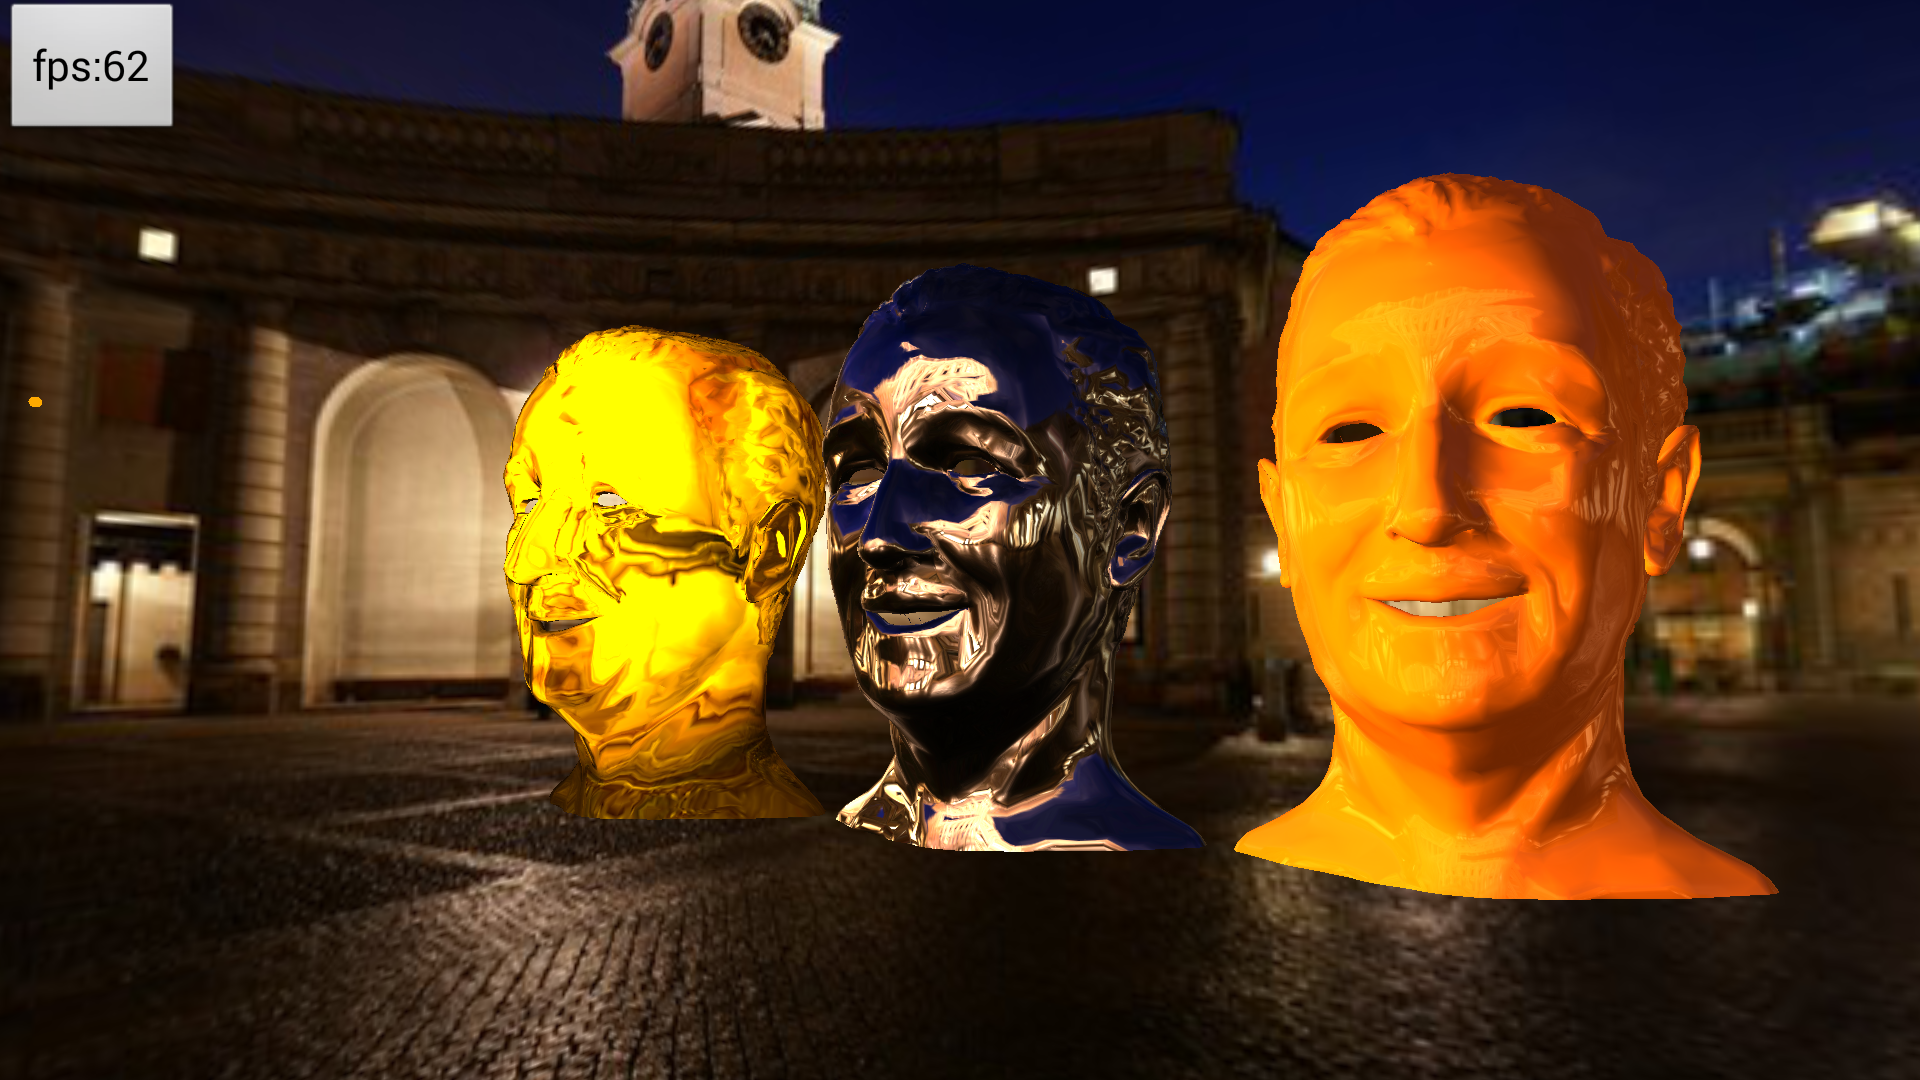
\includegraphics[width=1.0\textwidth]{webgl.png}
  \begin{tablenotes}
    \item This screen shot was taken from the CocoonJS Launcher Application on Android\footnotemark[16]
  \end{tablenotes}
\end{figure}

\footnotetext[16]{\url{https://play.google.com/store/apps/details?id=com.ideateca.cocoonjslauncher} - Accessed February 2014}

\subsection{Audio}
 Audio is a key component in delivering a satisfying game experience as it provides stimuli and feedback to the player. This can help further immerse the player in the game experience especially in main stream AAA games. Audio also plays a important part in mobile games, emphasising and cuing player interaction that would otherwise would require use of popups and explanatory text. These latter techniques are often avoided because they can bore and frustrate the player while breaking their immersion in the process, something which the does not apply to audio. Sound effects and music can serve as a branding mechanism that makes the company's other games easily recognisable to players. A good example of this is Rovio's \textit{Angry Birds} series, which often cross promotes games part of the series. It is important that the audio in mobiles games is subtle as anything abrasive to the player will almost certainly result in them muting or lowering the volume. Players have a very low tolerance levels for disturbing sound design, often a result of being conditioned by earlier mobile games on archaic devices. This stresses that audio must be used sparingly and in the appropriate context in order to deliver the full intended game experience \citep{Thomas}.

\subsubsection{HTML5 Audio}

The \texttt{<audio>} element is one of the significant addition from the HTML5 specification related to multimedia, alongside \texttt{<video>} and \texttt{<canvas>}. The purpose of this element is to define audio content within a HTML document by referencing an audio file. When the element is parsed by the browsers, it loads the referenced content similar to other elements (\texttt{<style>}, \texttt{<script>}), which can then be played back by web browsers internal media player. This element has enabled web applications to deliver audio to users natively, whereas before the advent of this element, they had to rely upon third-party plugins. Support for this element in mobile browsers is widespread; however, there are many discrepancies between them. Here is a list of some of the known issues that currently effect mobile browsers taken from \textit{caniuse.com}\footnotemark[17]:

\footnotetext[17]{\url{http://caniuse.com/\#feat=audio} - Accessed January 2014}

\begin{itemize}
  \item Audio played from the element in iOS always plays in a full screen player.
  \item Playback rate not supported on the stock android browser.
  \item Only one Audio file can be played at one time in iOS and Android browsers which forces you to use sprites for multiple audios.
  \item Audio in iOS can not be auto played. It even starts downloading after a user triggered event.
  \item Volume is read-only on iOS.
\end{itemize}

Much of these restrictions imposed by mobile web browsers make it difficult to utilise \texttt{<audio>} as an competent solution for dynamic sound effects and background music. This also poses a problem when trying to compete with native mobile games, as features like multichannel audio and equalizers come standard with their relative SDK.

\subsubsection{Web Audio API}
The Web Audio API is an experimental high-level JavaScript API that is currently being drafted and developed by Google and the W3C\footnotemark[18]. This API provides richer methods to manipulate and generate audio through signal processing and synthesis. This also includes the ability to load and playback audio files similar to the \texttt{<audio>} element. A similarly MediaStream API\footnotemark[19] developed by Mozilla is trying to achieve the same functionality focusing on the streaming of both audio and video related data.

\footnotetext[18]{\url{http://www.w3.org/TR/webaudio/} - Accessed January 2014}
\footnotetext[19]{\url{https://developer.mozilla.org/en-US/docs/WebRTC/MediaStream_API} - Accessed April 2014}

This appears to be a more appropriate technology for the implementation of game related audio. However, these technologies are much newer than the \texttt{<audio>} element and have yet to be implemented in any of the stock mobile browsers with the exception of iOS Safari versions \texttt{6.0-7.0}\footnotemark[20].

\footnotetext[20]{\url{http://caniuse.com/\#feat=audio-api} - Accessed May 2014}

\subsection{Tools}

\subsubsection{Node.js}
`Node.js is a platform built on Chrome's JavaScript runtime for easily building fast, scalable network applications. Node.js uses an event-driven, non-blocking I/O model that makes it lightweight and efficient, perfect for data-intensive real-time applications that run across distributed devices.'\footnotemark[21]. Essentially, it enables developers to program applications in JavaScript that are executed outside of a web browsers similar to other interpreted programming languages like Ruby and Python. Applications are written in the form of modules that rely on other modules. Core modules come bundled with the platform's binary and provide an API to common services such as HTTP and the File System. The NPM registry is where open-source and community created modules can be published alongside their dependencies. These self contained modules provide developers with even more utilities such as local development servers and build tools.

\footnotetext[21]{\url{http://nodejs.org/} - Accessed January 2014}

\subsubsection{Gulp}
Gulp\footnotemark[22] is a streaming build system for Node orientated development. Conventional build systems are configured through static data files that detail options as attribute-key pairs, such as XML and JSON. However, Gulp has innovated by enabling developers to configure their build tasks through a root JavaScript program labelled as \texttt{gulpfile.js}. The advantage of having build tasks configured in this way is that it enables utilisation other NPM modules. Essentially, Gulp streams source files in and out these modules, enabling the application to transform in a variety of combinations. Once the task of transforming is complete, the outputted files can be deployed to the file system. This streaming capability is enabled by Node.js, which is highly efficient compared to most build systems, since it never has to write temporary files to disk (everything is done at run-time using virtual file objects).

\footnotetext[22]{\url{http://gulpjs.com/} - Accessed May 2014}

\begin{figure}[h!]{A screenshot of the project's Gulp build output}
  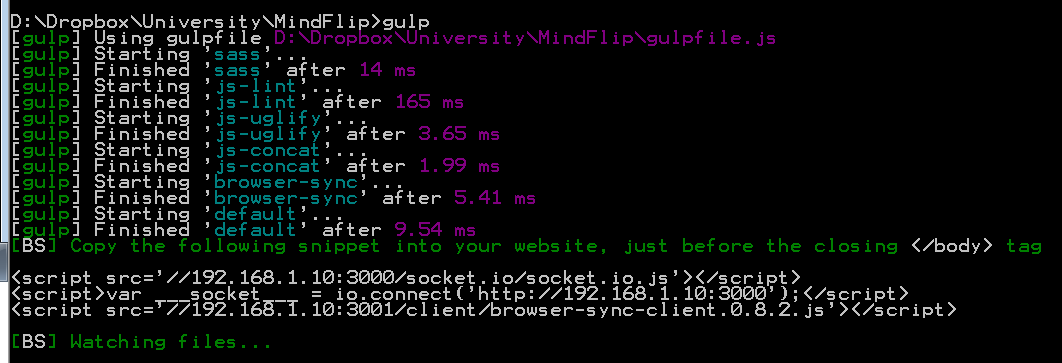
\includegraphics[width=1.0\textwidth]{gulp.png}
\end{figure}

\subsubsection{Bower}
`Bower\footnotemark[23] is a package manager for the web. It offers a generic, unopinionated solution to the problem of front-end package management, while exposing the package dependency model via an API that can be consumed by a more opinionated build stack. There are no system wide dependencies, no dependencies are shared between different apps, and the dependency tree is flat. Bower runs over Git, and is package-agnostic. A packaged component can be made up of any type of asset, and use any type of transport (e.g., AMD, CommonJS, etc.)' \citep{Twitter}. Essentially, it is very similar to the Node.js NPM registry utility, but instead of it being used for any kind of module, it just handles client-side tools and libraries utilised in most web applications. Bower has a better selection of libraries and plugins than the NPM registry because rules are not as strict.

\footnotetext[23]{\url{http://bower.io/} - Accessed May 2014}

\begin{figure}[h!]{A screenshot of the project's Bower list output}
  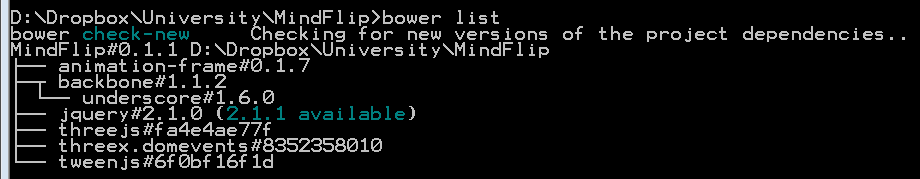
\includegraphics[width=1.0\textwidth]{bower.png}
\end{figure}

\subsubsection{Hybrid Mobile Application Frameworks}
Hybrid mobile applications are mobile web applications that run inside a native application container. The native application will instantiate a native web view and load the locally hosted web application simulating as if it were being loaded over a network. The advantage of having the web application hosted locally on the device is that no transfer actually takes place, as all the data that makes up the application will already be present on the device within the native application's assets. A \textit{WebView} is essentially the mobile OS's native web rendering engine used by the stock mobile browser, but without the unnecessary user interface required for navigating the Internet. Another advantage of running the web application encapsulated within a native application is the ability to bridge between the web application's JavaScript code to the OS's native API. This can enable access to native features such as the Camera and GPS. There are Web APIs developing ways to access these from JavaScript, but until these are widely implemented and supported, this bridge between web to native can fill in these gaps in support \citep{Smith}.

\subsubsection{weinre}
\label{sec:weinre}
`weinre'\footnotemark[24] (web inspector remote) is a debugger application created by Patrick Mueller\footnotemark[25], who is also a contributor to the Apache Cordova project. This application works similar to the built-in desktop browser debuggers and inspectors, with the added bonus of having a remote target. By including a remote JavaScript file hosted on a local weinre server, the mobile device can be linked, letting it send and receive debugger data from the server. This lets developers inspect and manipulate the mobile devices web browser. The key issue that prevented the further use of this application in the project's development was that in combination with Apache Cordova it was not able to log any information before the script was loaded and the console was initialized. Therefore, when it came to analysing the initial portion of an application's lifecycle, the data generated was restricted by this dependency.

\footnotetext[24]{\url{http://people.apache.org/~pmuellr/weinre/docs/latest/Home.html} - Accessed November 2013}
\footnotetext[25]{\url{http://muellerware.org/} - Accessed November 2013}

\section{Development}
\label{sec:dev}
The development process of HTML5 applications and games like the platform they are built on, is in constant flux with new methods, techniques, and tools surfacing all the time. Developers must ultimately choose a tooling stack that enables them to express their creativity, by letting them work productivity and efficiently. This undoubtedly will vary based on their personal preferences, background, and opinions on best practices. I have had no previous experience with HTML5 development, which encouraged me, during this project, to seek out the popular solutions to the problems I was encountering. This section of the report will detail the problems I faced, my found solutions, and what they let me accomplish. 

\subsection{Design}
I have had much experience with game design and development, but because of my inexperience with the HTML5 platform, I felt that the core concept of the game had to remain simplistic and allow for expansion. This choice was meant to ensure that the project remained feasible, as my self-education would likely consume the majority of this project's allotted time. After initial deliberation, I decided to base the game upon the simple card game of \textit{Concentration}\footnotemark[26] (also known as Pairs). The gameplay mechanics consist of the player initially being presented with several cards, each marked with a symbol linking it to a set. These symbols are only on the front-faces of the cards and are briefly visible to the player at the start of the game. When the cards are flipped the symbols are obscured, making each card indistinguishable from the rest. The player's objective is to identify the matching cards from memory. When designing a game it is important to be conscious of the player's perspective, as well as the flexibility it allows the developer. Hence, the following aspects of this game concept also made it an attractive candidate.

\footnotetext[26]{\url{http://en.wikipedia.org/wiki/Concentration\_(game)} - Accessed October 2013}

\begin{enumerate}
  \item The mechanics are simple, making it rapidly accessible for players of all ages to recognise and understand the core gameplay.
  \item It has depth, allowing for additional and more complex gameplay mechanics to be introduced gradually to the player.
  \item It will translate well to touch screens, as the fundamental interaction the player will have is selecting cards.
  \item It engages the player's brain in pattern recognition which is one of its inherent strengths.
\end{enumerate}

Other mechanics such as restricting the player to matching sets of cards in a particular order were later introduced to further challenge the player and keep them interested with an increasing difficulty curve. This engages other strengths of the player's brain, as they will have to chunk their memories of card positions and prioritize them so they can be retrieved later in a particular order. Subtle changes in level design such as introducing additional shapes and symbols in various symmetrical and asymmetrical patterns were also added to push the player's cognitive abilities.

\subsection{Implementation}

To get a head start on the project implementation I started researching and acquiring tools that provided a familiar development experience to what I was accustom to. I felt doing so would make my transition to JavaScript programming much faster than learning it from scratch. Much of my game development experience is from several years of building games for Adobe Flash using its ActionScript programming language, so I began looking at some of the popular transpiler languages that translate to JavaScript once compiled. Microsoft's TypeScript presented itself as a close alternative to ActionScript, with familiar syntax and features such as classes, interfaces, and typed variables, staples of conventional high-level languages. I installed the compiler using NPM (Node Packaged Modules), which is accessible through a command-line interface that comes as part of the \textit{Node.js} platform. After settling upon TypeScript as my intermediate language of choice I began testing various IDEs with TypeScript support. WebStorm a commercial JavaScript IDE featured, informative auto-completion, support for TypeScript with minimal configuration, and watchers (background processes that would compile TypeScript into JavaScript upon detecting changes). As a result of having my project supervisor fill out a request form, I was able to obtain an educational license for this IDE that would last the length of a year. Once comfortable with the development workflow of programming in TypeScript and compilation via WebStorm, I began implementing and testing the basic game logic using a tile map and object models that represented each card. After game logic was functional I began researching JavaScript graphics libraries that could offer a similar hierarchical pattern that I was acquainted with in AS3. This hierarchy revolves around subclasses of \texttt{DisplayObject} and \texttt{DisplayObjectContainer} that can be manipulated and organised through methods such as \texttt{addChild}, \texttt{removeChild}, and \texttt{setChildIndex}. These functions enable the grouping and layering of multiple visual elements such as images in local and global contexts.

CreateJS, is a suite of modular JavaScript libraries developed by Grant Skinner, sponsored by Adobe. This suite contains a library called EaselJS, that emulates the aforementioned pattern, while also providing other useful APIs for asset loading, visual effects, masking, transforms, and mouse interaction. EaselJS can render this display list hierarchy setup via programming and renders its children to a HTML5 Canvas. During this period of research, I also came across the Apache Cordova project which also provided a command-line tool through \textit{NPM}. Using EaselJS and Cordova I managed to develop and deploy a rough prototype of the game from placeholder art and the initial game logic I had already programmed in TypeScript. Unfortunately, working with the CreateJS suite in combination TypeScript proved to be more challenging than I initially thought. Moreover, the performance of HTML5 Canvas was slow and stuttering in Cordova, which further made me reconsider this approach. In order to fully utilise the features of TypeScript in combination with a typical JavaScript library, TypeScript definitions are required. TypeScript definitions outline a JavaScript library's API with type annotations in \texttt{.d.ts} files similarly to \texttt{.h} header files in C++. These \texttt{.d.ts} files can be referenced, which help the compiler map between TypeScript and JavaScript enabling features such as compile-time error detection and auto-complete in the IDE. There is an open source repository maintained by the TypeScript community on GitHub called DefinitelyTyped\footnotemark[27] , which does contain definition files for the CreateJS libraries. However, upon further inspection I found the definition files were obsolete and incompatible with the latest version of CreateJS. The time it would have taken for me to manually correct the definitions to get them to up-to-date would have been a lengthy process. I also felt that working at this level of abstraction above the true underlying JavaScript could potentially hinder my ability to debug later in development. This ultimately led to the abandonment of EaselJS and TypeScript in favour of migrating to JavaScript and DOM orientated approach.

\footnotetext[27]{\url{https://github.com/borisyankov/DefinitelyTyped} - Accessed October 2013}

While educating myself in JavaScript I found the lack of built-in structure daunting, and was worried it could plague my project's development as I lacked experience with the language. After further research I chose to employ the use of a JavaScript \textit{MV*} framework as it provided a structured pattern in which to develop a web application. I selected Backbone.js\footnotemark[28] because of its flexibility, large community following, and modular design. As described in a presentation given by \citet{Bull} Backbone.js is the equivalent of a \textit{knife/spoon/fork} on a camping trip. This analogy emphasises its modularity, implying that there is no imposed exclusivity between its internal components. This allowed me to gradually implement the use of its Model, View, Collection, and Router classes throughout this project's development, without being forced to learn everything at once but only when it was required. I began using Backbone, first, by porting my game logic code into appropriate \textit{Model} classes and my EaselJS/HTML5 Canvas code to \textit{View} classes that instead employed the use of the DOM.

\footnotetext[28]{\url{http://backbonejs.org/} - Accessed December 2013}

Several improvements arose after the switch from rendering on Canvas to utilising the DOM. For instance, the original implementation of the card flip effect was achieved by simply tweening the width of the images to 0 and back. This technique produced a very flat effect. After switching from this Canvas implementation to using DOM elements, I was able to make use of CSS3 transforms. These transforms allow for 3D manipulation one area that the EaselJS library was lacking in. This allowed me to add perspective to the flip effect, which made it more aesthetically pleasing and helped highlight the user's interaction. The transition could be applied through adding and removing a CSS class selector to and from a particular card's DOM element. CSS3 transforms are hardware accelerated on many mobile devices, making the animation smoother than with the previous implementation. Also, because the browser handled process of rendering, it applied anti-aliasing by default making the edges of the images less jagged.

\begin{figure}[h!]{A comparison of original flip effect and current flip effect (left-to-right)\label{transforms}}
  
\includegraphics[width=1.0\textwidth]{transforms.png}
\end{figure}

Scaling the game's visual elements to fit the varying screen sizes of my mobile devices proved more challenging in the DOM than it had been with the use of a Canvas element. The original scaling process consisted of setting the Canvas element's dimensions to match that of the window upon it firing a \texttt{resize} event, then updating the scale properties of the EaselJS \texttt{stage} instance appropriately. However, when working with the DOM, every element is rendered and positioned in the page's layout relative to its style attributes (such as \texttt{display}, \texttt{position}, and \texttt{float}), which means that almost all the rendering of the game's visuals could only be influenced indirectly. I first attempted to scale my game using \textit{viewport units}, which lets you set elements style attributes relative to the current viewport's dimensions. For example, \texttt{width:50vh} would make an element's width 50\% of the viewport's height. However, I found that the majority of stock mobile web browsers had not yet implemented this feature, with it only being present in versions 4.4 of Android and 6.0 of iOS (see Figure \ref{viewport}). This led me to seek an alternative solution that could give me a similar effect.

\begin{figure}[h]{A compatibility table of support for viewport units \label{viewport}}
  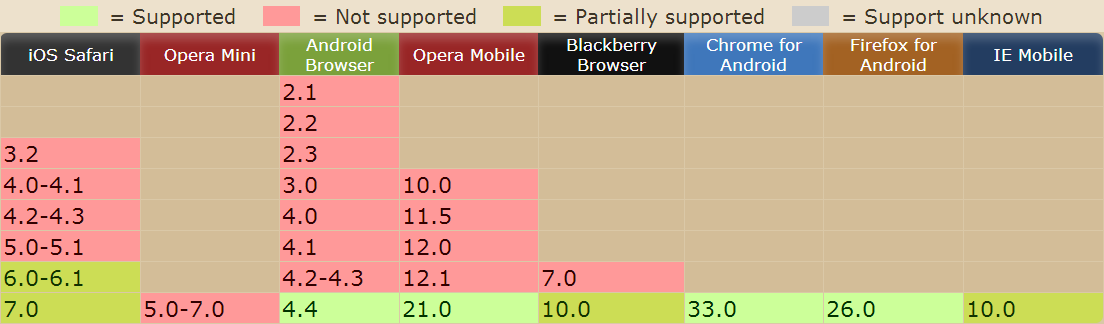
\includegraphics[width=1.0\textwidth]{viewportunits.png}
    \begin{tablenotes}
      \item Source: \url{http://caniuse.com/\#feat=viewport-units}\\ Accessed November 2013
    \end{tablenotes}
\end{figure}

Remote debugging was a task I frequently had to perform in order to analyse problems that occurred while running on mobile. It was important to find a solution that was efficient and compatible with Cordova hybrid mobile applications. After searching for tools that fitted this criteria, I discovered the weinre project. I have explained in a section \ref{sec:weinre} how this software works in detail. I stuck with this solution for a large chunk of development because nothing better was available at the time, although launching the local weinre server, connecting my mobile devices, and then navigating to the inspector's interface through a browser on my desktop computer, was an arduous process. Later in development, I discovered that Google Chrome comes with built-in `DevTools' that feature remote inspection of an Android Web View, providing it was using the latest OS (4.4 KitKat). This solution significantly improved my development process making it rapidly iterative. First I would debug the game in Chrome on my desktop computer. If all went well, I would then build, deploy, and launch the application on mobile through Cordova's command-line interface, which automatically connected to the familiar Chrome's DevTools I had just used, to test the desktop version. Chrome also later added mobile emulation to DevTools which facilitated the simulation of touch events, device orientation, and screen density/resolution. This was preferable to deploying the Cordova package everytime I wanted to quickly test mobile functions, as it loaded quicker than the time it took to build and deploy the package to mobile. However, I still tested on mobile at regular intervals to ensure overall compatibility.

As the project progressed, the addition of numerous tools and libraries meant that the structure and build processes grew overly complicated, which diminished my ability to implement efficiently. Many of these tools and libraries the project relied upon were NPMs in the Node.js ecosystem, which led me to the conclusion that I should also format my project as a NPM. NPMs are configured through their \texttt{package.json} file in the project's root directory. In this file, I was able to specify the dependencies of my project and define scripts that ran a variety of tasks such as launching the local development server or deploying the mobile game through Cordova.

As I added more levels to the game I decided to implement the locking of future levels similar to that of most popular mobile games. This unlocking of levels acts as a reward system that the player can become invested in, encouraging them to come back. However, this came with the overhead of storing persistent data that would maintain their progress between play sessions. HTML5 Local Storage provided a quick cross-platform solution that allowed for the storing of key value pairs on the player's device without interacting with native APIs. I used this to store level data, that included a boolean value representing the locked/unlocked state, as well as all the scores obtained by the player. Once deployed on the centralised app stores I plan to sync this data with a player account so they can compare scores with others, adding a competitive element to their progression.

Nearer the end of the project I became aware of 

After reaching the end of the implementation process, I had integrated several more project development tools. The final project structure relied upon using NPM to manage all the development tools such as Apache Cordova, Bower, and Gulp.js. Cordova was used to wrap the HTML5 game as a native application. Bower, the package manager, was used to organise all my front-end libraries used by the HTML5 application such as Backbone.js and jQuery. Finally, everything was tied together by \textit{Gulp.js}, a streaming build system that managed all my project tasks such as bundling the game modules and front-end libraries, minifying and obfuscation of the bundles for release, building the Cordova application from the HTML5 application source, and deploying the built application to mobile devices.

\subsection{Feedback}
Throughout the development of my game, I considered it essential to obtain feedback and reactions from players to gauge its performance first hand. Therefore, whenever willing participants were available, such as friends, family, and classmates, I presented them with a device containing the latest stable build, and observed their behaviour to get third-party perspective. To test the intuitiveness, I gave them no explanation or hint as to how the game should be played. Indeed, the process a player goes through in order to understand the mechanics is a vital component of player satisfaction. If they do not understand the game's rules almost instantaneously, many people will lose interest shortly after picking it up.

The first playable prototype received a lot of feedback from players relating to `lag'. The `lag' they were referring to was the latency between their interaction and visual/audible feedback. This gap detracts from the responsiveness and tactile impression required to inform the player. After some research I found an article written by \citet{Croft} on creating responsive buttons with PhoneGap (Cordova), which encouraged me to test different JavaScript events. I found that \texttt{touchstart} and \texttt{touchend} events fired much faster than the \texttt{click} event, I was currently using. This is intentional because mobile browsers delay the firing of the \texttt{click} event, in order to differentiate it from the initial press which is represented by the \texttt{mousedown} and \texttt{touchstart} events. There are plans of unifying these two sets of events under the a pointer events specification, but until this is implemented by browser vendors developers have to deal with this fragmentation. I solved this problem for both platforms by employing a feature detection library that let me choose which events to listen for upon initialisation. Another optimization I made was to keep the style of the buttons to a minimum, as complex effects take longer to render which happens every time the button changes state. These modifications solved the latency of visual feedback. I tackled the audible latency by analysing the waveform of the sound effects that were sourced from \textit{freesound}. I found many of the sound effects had a lot of trailing blank space at the beginning and ends of the audio files, so after trimming, fading, and normalizing all the effects, this decrease a significant portion of the latency. However, after further play tests it was apparent there was still a minor delay between the event firing and the audio playing. I thus decided to switch from HTML5 Audio to a Cordova's official Media plugin that gave me access to native audio capabilities. Web Audio API would have been a preferable alternative but most mobile browsers had yet to implement it. Unfortunately, the offical Media plugin still had quite a high latency. After searching I found a custom \textit{LowLatencyAudio} plugin that had been developed by \citet{Trice} for the PhoneGap framework (the predecessor of Cordova). Since its debut, the plugin has been ported to for Cordova by \citet{Xie}, but only for Android and iOS, which finally brought the audible latency to a reasonable level.

When repeatedly testing, developers can become accustomed with the game, which leads them to underestimate the game's accessibility to new players. This often takes the form of unintentionally assuming prior knowledge on part of the player. In some cases, this can have a positive effect, allowing them to skip explanation of common tropes by drawing parallels to that of other popular games. A good example is the match-three game popularised by \textit{Bejeweled} in the 2000s. After its debut, this same mechanic has surfaced again in the popular mobile game \textit{Candy Crush Saga}, which has innovated, adding further complexity to a familiar concept \citep{Juul}. Leveraging existing tropes can act as a shortcut when teaching a player new or similar game systems. Nonetheless, these can also be stumbled upon accidentally from a developer's perspective, as their preconceptions will often differ vastly by comparison to the average player. This was the case of the introductory level in my initial draft. At the start, the first two symbols the player encountered were a red nought and a blue cross on a three-by-three grid. During the first play test of this level, I discovered the player's natural instinct was complete the level by producing a winning \emph{Tic-tac-toe} game state. This was a glaring flaw in my game's design, because the symbols are common to a pre-existing game (namely \emph{Tic-tac-toe}). The player receives mixed signals about how to play the game from the offset, leading to confusion and ultimately, frustration. I thus later decided to try a simpler approach, using more abstract symbols (such as circles, squares, and triangles) in my initial set of levels. These symbols are more generic and therefore do not have any strong associations that can mislead the player.

When repeatedly testing, developers can become accustomed with the game, which leads them to underestimate the game's accessibility to new players. This often takes the form of unintentionally assuming prior knowledge on part of the player. In some cases this can be used to their advantaging allowing them to skip explanation of common tropes by drawing parallels between their game's mechanics and that of other popular games. A good example is the match-three game popularised by \textit{Bejeweled} in the 2000s, this same mechanic has surfaced again in the popular mobile game \textit{Candy Crush Saga} who have innovated adding further complexity to a familiar concept \citep{Juul}. Leveraging existing tropes can act as a shortcut when teaching a player new or similar game systems. However, these can also be stumbled upon accidentally from a developer's perspective as their preconceptions will often differ vastly by comparison to the average player. This was the case of the introductory level in my initial draft. At the start, the first two symbols the player encountered were a red nought and a blue cross on a three-by-three grid. During the first play test of this level, I discovered the player's natural instinct was complete the level by producing a winning \emph{Tic-tac-toe} game state. This was a glaring flaw in my game's design, because the symbols are common to a pre-existing game (namely \emph{Tic-tac-toe}), the player receives mixed signals about how to play the game from the offset, leading to confusion and ultimately frustration. I thus later decided to try a simpler approach, using more abstract symbols, such as circles, squares, and triangles in my initial set of levels. These symbols are more generic and therefore do not have any strong associations that can mislead the player.

\section{Conclusion}
During the past year spent carrying out this project, the amount of emerging tools and technologies for developing cross-platform HTML5 mobile applications has figuratively exploded. This variety of options has made the development of my game very challenging. As soon as I settled upon a development stack and workflow, a more optimal approach emerged. I have had to perpetually research these new approaches, assessing whether they presented a better alternative to that of what I was currently using. Every time I made a switch to one of these better alternatives, I have had to expend time and energy in learning and integrating it into my existing project. I am hopeful that in the near future, when the HTML5 specification starts to solidify, support for its full feature will be widespread amongst all web browsers. This project was not a commercial endeavour, which allowed me to afford the freedom to incorporate and substitute components of my project at will, when superior alternatives were at hand. However, in the context of commercial development, it is likely that locking down a project's tools and dependencies once it reaches maturity would be a more sensible decision. Regardless of this constantly switching context, the allowance of which was a choice on my part, the project has delivered a cross-platform mobile game built using HTML5. This game is proof of concept that to have every platform version stem from a single project highly increases development efficiency over that of native development. If a company chooses to develop a mobile application natively, they will require several developers, each to program a native variant of the application while stay consistent, which can be a mammoth task as each mobile operating systems requires a different programming language and skill set (iOS uses Objective-C, Android use Java, Windows Phone uses C\#). This project did not have a team of developers at its disposal, only me; I have managed to produce a functional game working with just the Web Platform, a platform I had no experience with prior to the beginning of this project. This is almost entirely due to the fact that one change made to the game's code or assets will instantly be reflected in all of its exported mobile applications. Overall, I feel this project has been a success. Despite the challenges I faced, the game is exactly what I had envisioned - a simple game with room for innovation.
For this platform to be widely adopted by mobile game developers, mobile vendors need to invest more resources that would contribute to the integration of web applications into their mobile ecosystem. If HTML5 applications were publishable through the vendors' mobile application stores without the use of hybrid frameworks, it would provide an acquisition (browser, install, launch) experience for users that does not differentiate from that of conventional native applications'. WebGL will likely become the best way to deliver and render gaming experiences through HTML5, but until it is widely supported, developers have to rely on hybrid frameworks that provide a fall-back solution.
In hindsight I would have invested more of my game development in WebGL, but at the time there was almost no support for it, even with hybrid frameworks. Support for WebGL increased rapidly over the course of development, with solutions such as CocoonJS and even Chrome and Firefox for Android supporting it as of their latest release. Going forward, I plan to develop the game further by porting the code to use Google's Dart, WebGL, and CocoonJS, and I may then go on to publish it officially on the Google Play Store.

\section{Future}
The key issue HTML5 is tackling on the mobile platform is portability. OEMs will continue to improve and innovate their product lines at different rates relative to what is profitable and marketable. As the cost of the technology required to construct these devices plummets, so does the cost to improve and innovate. The technology life-cycle of mobile devices is short in contrast to that of web specifications. If developers desire to achieve cross platform compatibility, there are many moving targets they have to hit when it comes to native development: hardware specifications, operating systems, store requirements, and official software development kits. Hitting these targets in a constantly fluctuating landscape demands much of a developer's focus, which could be better spent more effectively improving a game's overall quality and design. The web has proved itself as a stable and universal platform on desktop computers, and, eventually, this will be implemented fully on mobile devices.

Currently, the platform on mobiles is lacking full support of accelerated canvas and WebGL in stock mobile browsers. However, this does not have to discourage developers as the support is on its way. In the mean time, developers can use hybrid mobile application frameworks such as Apache Cordova and CocoonJS to get a head start on utilising this `edge' feature. Once native support for these features is introduced, their original source code will be inherently compatible, not even requiring compilation. As processing power on mobile devices increases, other concerns, such as performance, will eventually become irrelevant and the developers' focus will skew towards the architecture and accessibility of their code rather its over engineered optimisation.

The future of JavaScript looks bright according to the creator \citet{Eich}. ECMAScript 7 intends to introduce language features such as overloadable operators, observers, value objects, and SIMD (single instruction, multiple data) intrinsics. The use of SIMD and low-level value objects in JavaScript will lead to near native performance while being widely compatible across processor architectures such as Intel's SSE, AMD's AVX, and ARM's NEON popularly used in mobile devices. He goes on to promote his extensible web manifesto\footnotemark[29] that notably focuses on adding safe and secure low-level capabilities to the web platform, as well as simplifying and streamlining the standardisation process by tightening the feedback loop between committees and developers.

\footnotetext[29]{\url{http://extensiblewebmanifesto.org/} - Accessed May 2014}

The video games industry will continue to grow in scope. Consoles such as the \textit{Nintendo Wii} have had widespread success across demographics in recent years. Such victories are bringing this creative medium to mainstream society. I feel mobile devices will similarly perpetuate the medium as they become common place in our daily lives. With the web growing alongside these devices it is a natural progression that they become intertwined. This is already happening in projects such as Ubuntu for Phones and Firefox OS. The web platform presents attractive prospects for game developers, offering lasting portability, which, as performance issues become less of a problem, will become their dominant priority. This project has encouraged me to seek out and research this platform thoroughly. I believe that my newly acquired skills and experience will hugely useful going forward with my career in industry.

\clearpage
\bibliography{5939968}

\end{document}

